\section{Comparison of FIX and Standard Preprocessing}\label{sec:comp}

The following section will present the results using both the standard preprocessing pipeline and FIX pipeline. First, activation related to the 48$^\circ$ C stimuli, achieved from using both methods is presented. Secondly, the difference in the amount of activation achieved by using FIX compared to standard preprocessing will be presented. \\
As mentioned in \secref{sec:stats}, a within heat run, within participant and within group analysis were run on the preprocessed fMRI data. Only the within group analysis will be presented in the results section. \Figref{fig:res:stdpos} and \figref{fig:res:stdneg} show the intensity of activation and the localization of the positive and negative activation achieved using the standard preprocessing pipeline. The figures will include a slice-wise illustration of the main areas of interest. The areas of interest will only be illustrated in the first two figures.     


\begin{figure}[H]                 
	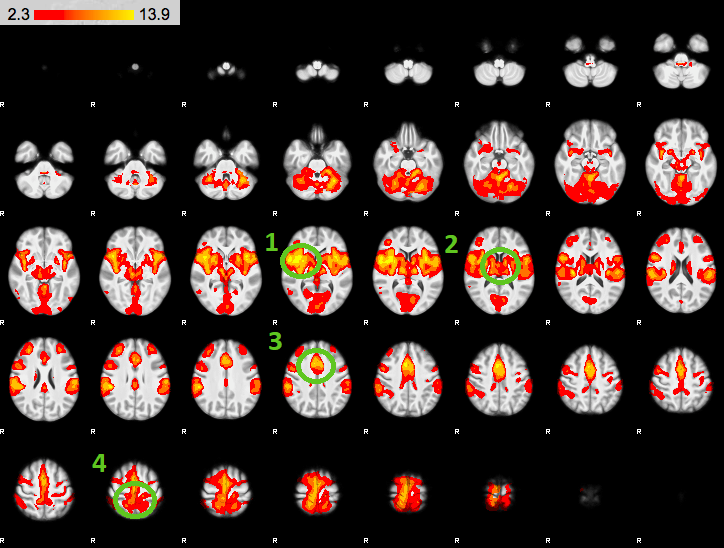
\includegraphics[width=.65\textwidth]{figures/Results/STD_pos_1}  
	\caption{Results of the achieved positive brain activation after using standard preprocessing, which yielded a Z-score range of 2.3 to 13.9. The activation is mainly localized in the regions of the insular cortex (1), basal ganglia (2), anterior cingulate cortex (3), and primary and secondary sensorimotor cortices (4).}
	\label{fig:res:stdpos} 
\end{figure}

\begin{figure}[H]                 
	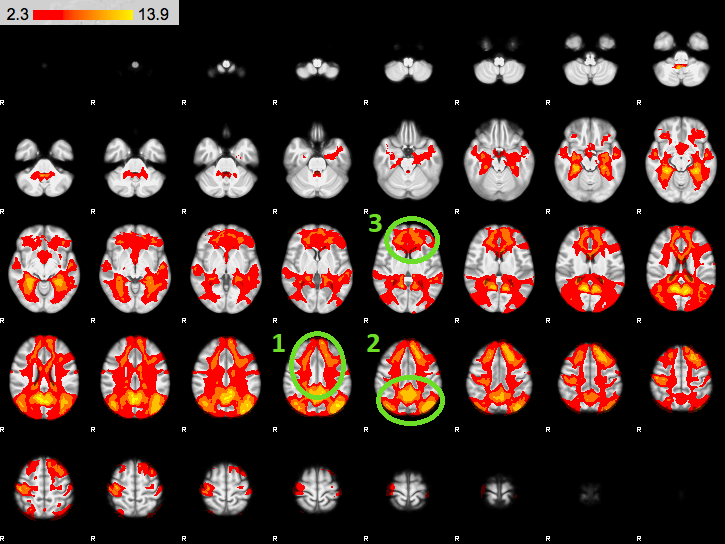
\includegraphics[width=.65\textwidth]{figures/Results/STD_neg_1}  
	\caption{Results of the achieved negative brain activation after using standard preprocessing which yielded a Z-score range of 2.3 to 13.9. The negative activation is mainly localized in the white matter (1) and the default mode network (posterior cingulate cortex (2) and prefontal cortex (3)).}
	\label{fig:res:stdneg} 
\end{figure}

The localization of regions which are activated during the noxious heat stimuli are primarily those associated with noxious stimuli as presented in \secref{sec:pain}. The main activation is localized in the regions of the insular cortex, basal ganglia, anterior cingulate cortex, and the primary and secondary sensorimotor cortices. %The Z-score range of the map has a range 2.3 to 13.9. \\
\Figref{fig:res:FIXpos} and \figref{fig:res:FIXneg} show the intensity of activation and localization of the positive and negative activation achieved using the FIX preprocessing pipeline. 

\begin{figure}[H]                 
	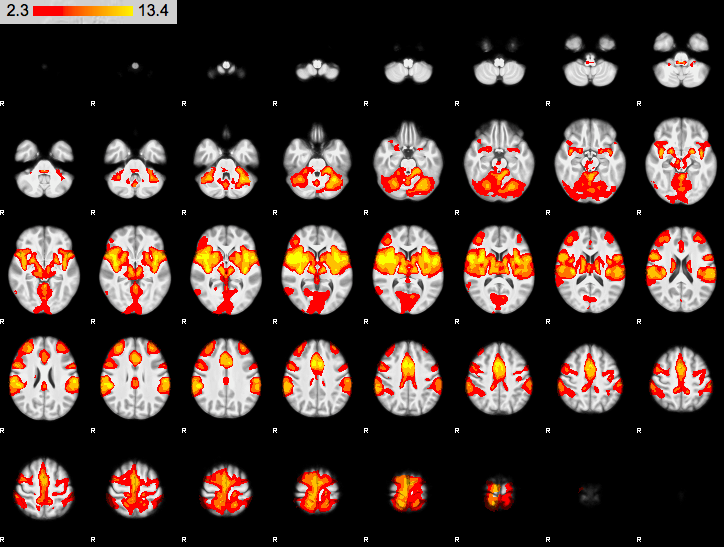
\includegraphics[width=.65\textwidth]{figures/Results/FIX_pos}  
	\caption{Results of the achieved positive brain activation after FIX preprocessing which yielded a Z-score range of 2.3 to 13.4. The activation is mainly localized in the regions of the insular cortex, basal ganglia, anterior cingulate cortex, and primary and secondary sensorimotor cortices.}
	\label{fig:res:FIXpos} 
\end{figure}

\begin{figure}[H]                 
	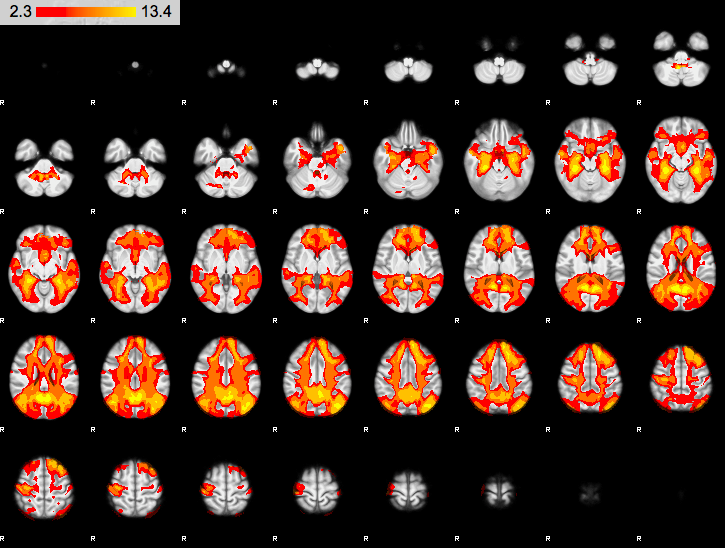
\includegraphics[width=.65\textwidth]{figures/Results/FIX_neg}  
	\caption{Results of the achieved negative brain activation after FIX preprocessing which yielded a Z-score range of 2.3 to 13.4. The negative activation is mainly localized in the white matter and the default mode network.}
	\label{fig:res:FIXneg} 
\end{figure}

The localization and intensity of the activation found by using FIX were similar to the one seen using standard preprocessing. %The Z-score range is though a bit less as it ranges from 2.3 to 13.4.
The results of using the standard preprocessing pipeline and FIX pipeline were very similar for both the positive and negative activation maps.   
To get a statistical measure of the differences in localization and intensity between the two preprocessing methods a comparison was made. \Figref{fig:res:diff_pos} shows where activation is greater for the FIX preprocessed data compared to the standard preprocessed data, and \figref{fig:res:diff_neg} shows where activation is greater for the standard preprocessed data compared to the FIX preprocessed data.

\begin{figure}[H]                 
	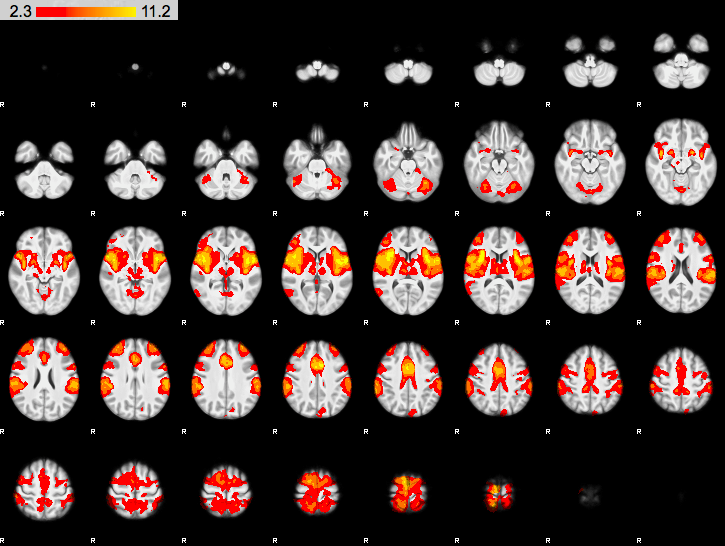
\includegraphics[width=.65\textwidth]{figures/Results/diff_pos}  
	\caption{Results from the comparison of the two preprocessing methods for noise removal. The activation seen is the intensity gained with using FIX compared to using standard preprocessing which yielded a Z-score range of 2.3 to 11.2. Increased signal is mainly seen in the insular cortex, anterior cingulate cortex and basal ganglia.}
	\label{fig:res:diff_pos} 
\end{figure}

\begin{figure}[H]                 
	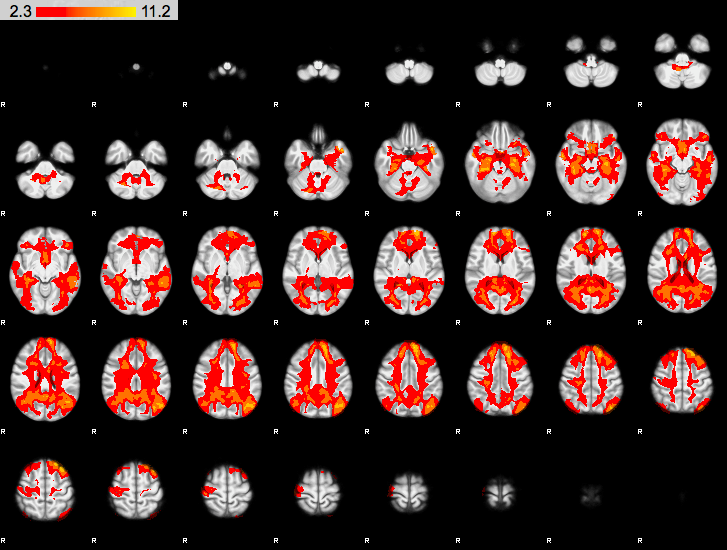
\includegraphics[width=.65\textwidth]{figures/Results/diff_neg}  
	\caption{Results from the comparison of the two preprocessing methods for noise removal. The activation seen in the image is the amount of activation which have been removed by using FIX compared to standard preprocessing which yielded a Z-score range of 2.3 to 11.2. Areas where activation had been lowered were white matter and default mode network.}
	\label{fig:res:diff_neg} 
\end{figure}
Examining figure 5.5 and 5.6 it could be deduced that the use of FIX preserved more signal of interest while lowering the amount of activation in areas of no interest compared to using standard preprocessing. The most dominant activation in areas of interest was seen in the insular cortex, anterior cingulate cortex and basal ganglia, while default mode network and white matter activation was lowered.
To summarize the results of using FIX compared to solely using standard preprocessing, a larger amount of signal related to the 48$^\circ$C noxious heat stimuli was achieved using FIX, thus preserving more signal of interest. Thereby, more signal of no interest had been lowered using FIX compared to standard preprocessing. 
